\chapter{Архитектура 32-х разрядного процессора RISC-V}

\section{Особенности семейства RISC-V}

Принципы RISC:
\begin{itemize}
    \item отсутствие вычислительно сложных инструкций;
    \item фиксированная длина инструкции;
    \item большое количество регистров общего назначения;
    \item ограничения на работу непосредственно с оперативной памятью как с медленным устройством.
\end{itemize}


\section{Форматы команд}

Процессор содержит:
\begin{itemize}
    \item 32 регистра общего назначения, доступа к специализированным регистрам нет (в т. ч. нет регистра флагов, даже на аппаратном уровне!);
    \item 4 базовых типа команд (рисунок~\ref{command-01}):
    \begin{itemize}
        \item \textbf{R} --- типа «регистр-регистр-регистр» (Register)
        \item \textbf{I} --- типа «непосредственное значение-регистр-регистр» (Immediate)
        \item \textbf{S} --- типа «регистр-регистр-непосредственное значение» (Store)
        \item \textbf{U} --- типа «непосредственное значение-регистр» (Upper)
    \end{itemize}
    \item
    \item
    \item
    \item
    \item
\end{itemize}

\begin{figure}[htbp]
    \centering
    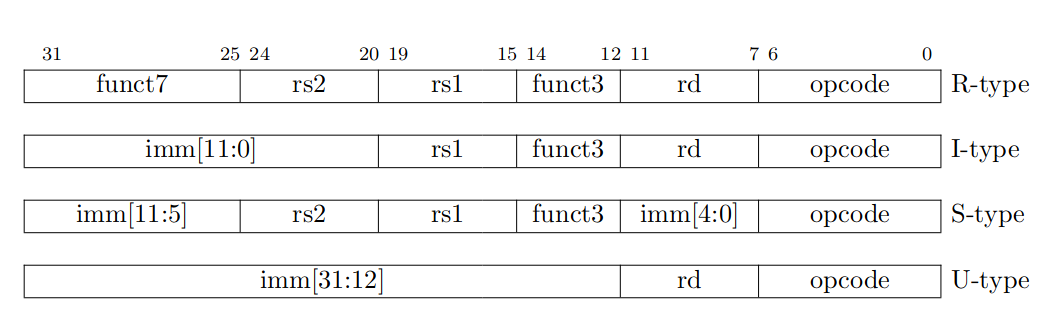
\includegraphics[width=1.0\textwidth]{img/RISCV_4_Commands.png}
    \caption{Основные форматы команд 32-разрядного процессора RISC-V}
    \label{command-01}
\end{figure}
Обозначения на рисунке:
\begin{itemize}
    \item \textbf{opcode} — код операции (6 битов)
    \item \textbf{rs1} --- № регистра-источника (5 битов)
    \item \textbf{rs2} --- № регистра-опреанда (5 битов)
    \item \textbf{rd} --- № регистра-приёмника (5 битов)
    \item \textbf{imm[11:0]} --- непосредственный операнд размером в 12 битов (В случае, когда непосредственное значение определяет «приёмник» (смещен адреса для «близкого» перехода или записи результата в память), 12 битов целиком в поле rd не помещаются, и его приходится «распиливать» (инструкция типа S). Непосредственный операнд всегда знаковый, и его знак всегда приходится на 31-й бит)
    \item \textbf{imm[31:12]} --- непосредственный операнд размером в 20 битов. Используется в инструкциях типа U для заполнения старших двадцати битов регистра (в операциях «далёкого» перехода и как дополнительная инструкция при записи в регистр полного 32-разрядного непосредственного операнда)
    \item \textbf{funct} --- поле функции (6 битов), используется для разных инструкций, у которых код операции одинаковый. Например, все арифметические инструкции типа I имеют одинаковый opcode OP-IMM (чему он равен?), а различаются полем funct. По-видимому, для эффективной реализации R-команд в конвейере удобнее не декодировать опкод, а по-быстрому сравнить его с нулём, и получать значения регистров, параллельно декодируя функцию, чтобы потом её применить.
\end{itemize}

\debate[Примечание]{Ниже представлен альтернативных рисунок из Reference Card с большим числом форматов. На всякий случай. Просто ряд форматов имеют одинаковые поля, но различную семантику. Пока непонятно, что лучше и проще преподносить. Может сказать о второй форме как способ уточнения семантики?}

Щесть базовых типов команд (рисунок~\ref{command-02}):

\begin{figure}[htbp]
    \centering
    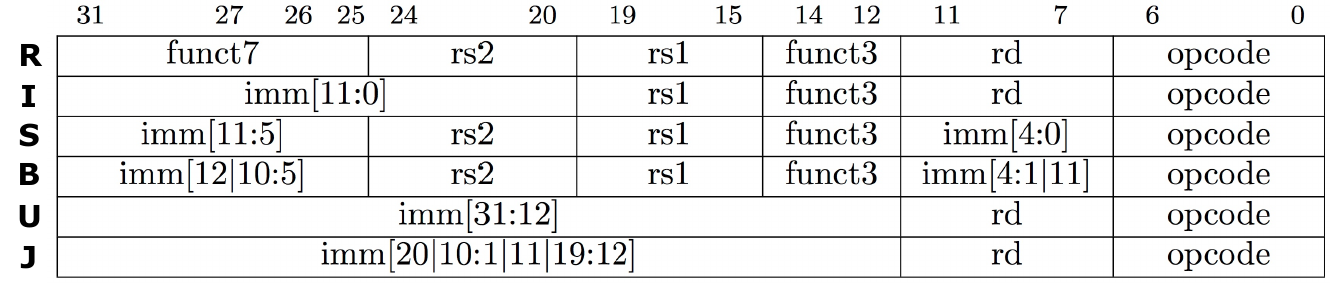
\includegraphics[width=1.0\textwidth]{img/32-bit-instruction-formats.png}
    \caption{Основные форматы команд 32-разрядного процессора RISC-V}
    \label{command-02}
\end{figure}

\section{Базовый набор команд процессора}

Процессор содержит основной набор команд, каждая из который отображается в одну инструкцию на языке ассемблера. Вместе с тем ассемблер, для повышения удобства программирования, дополнительно поддерживает псевдокоманды, каждая из которых может кодировать до нескольких машинных команд или иметь специфические операнды, позволяющие сформировать мнемонику команды, удобную для восприятия человеком.

Арифметические команды представлены в таблице~\ref{table-base-arithmetic}

\begin{table}[h]
    \caption{Арифметические команды набора RV32I}
    \centering
    \begin{tabularx}{\textwidth}{|l|c|X|}
        \hline
        \textbf{Команда} & \textbf{Формат} & \textbf{Описание} \\
        %\hline  \multicolumn{3}{|c|}{\textbf{\textit{Арифметические}}} \\
        \hline \verb|add rd,rs1,rs2| & R & Целочисленное сложение: \verb|rd  = rs1 + rs2| \\
        \hline \verb|addi rd,rs1,int12| & I & Сложение непосредственно с числом: \verb|rd = rs1 + int12| \\
        \hline \verb|sub t1,t2,t3| & R & Subtraction: set t1 to (t2 minus t3) \\
        \hline \verb|lui t1,100000| & U & Load upper immediate: set t1 to 20-bit followed by 12 0s \\
        \hline \verb|auipc rd,100000| & U & Сложение старших 20 разрядов непосредственного числа с \verb|pc|: \verb|rd = pc + int[31:12]| (pc плюс 20-бит непосредственного операнда как старшие разряды 32-разрядного числа, расширенного нулями) \\
        \hline
    \end{tabularx}
    \label{table-base-arithmetic}
\end{table}

Логические команды представлены в таблице~\ref{table-base-logical}

\begin{table}[h]
    \caption{Логические команды набора RV32I}
    \centering
    \begin{tabularx}{\textwidth}{|l|c|X|}
        \hline
        \textbf{Команда} & \textbf{Формат} & \textbf{Описание} \\
        %\hline  \multicolumn{3}{|c|}{\textbf{\textit{Арифметические}}} \\
        \hline \verb|add rd,rs1,rs2| & R & Целочисленное сложение: \verb|rd  = rs1 + rs2| \\
        \hline \verb|addi rd,rs1,int12| & I & Сложение непосредственно с числом: \verb|rd = rs1 + int12| \\
        \hline \verb|sub t1,t2,t3| & R & Subtraction: set t1 to (t2 minus t3) \\
        \hline \verb|lui t1,100000| & U & Load upper immediate: set t1 to 20-bit followed by 12 0s \\
        \hline
    \end{tabularx}
    \label{table-base-logical}
\end{table}


Команды сдвига представлены в таблице~\ref{table-base-shift}

\begin{table}[h]
    \caption{Команды сдвига набора RV32I}
    \centering
    \begin{tabularx}{\textwidth}{|l|c|X|}
        \hline
        \textbf{Команда} & \textbf{Формат} & \textbf{Описание} \\
        \hline \verb|xor t1,t2,t3| & R & Bitwise XOR : Set t1 to bitwise XOR of t2 and t3 \\
        \hline \verb|xori t1,t2,-100| & I & Bitwise XOR immediate : Set t1 to bitwise XOR of t2 and sign-extended   12-bit immediate \\
        \hline \verb|or t1,t2,t3| & R & Bitwise OR : Set t1 to bitwise OR of t2 and t3 \\
        \hline \verb|ori t1,t2,-100| & I & Bitwise OR immediate : Set t1 to bitwise OR of t2 and sign-extended 12-bit immediate \\
        \hline \verb|and rd,rs1,rs2| & R & Поразрядное И: \verb|rd = rs1 & rs2| \\
        \hline \verb|andi rd,rs1,int12| & I & Поразрядное И непосредственно с числом: \verb|rd = rs2 & int12| (с расширением знакового разряда у int12) \\
        \hline
    \end{tabularx}
    \label{table-base-shift}
\end{table}

Команды сравнения представлены в таблице~\ref{table-base-compare}

\begin{table}[h]
    \caption{Команды сравнения набора RV32I}
    \centering
    \begin{tabularx}{\textwidth}{|l|c|X|}
        \hline
        \textbf{Команда} & \textbf{Формат} & \textbf{Описание} \\
        \hline \verb|slt t1,t2,t3| & R & Set less than : If t2 is less than t3, then set t1 to 1 else set t1 to 0 \\
        \hline \verb|slti t1,t2,-100| & I & Set less than immediate : If t2 is less than sign-extended 12-bit immediate, then set t1 to 1 else set t1 to 0 \\
        \hline \verb|sltu t1,t2,t3| & R & Set less than : If t2 is less than t3 using unsigned comparision, then set t1 to 1 else set t1 to 0 \\
        \hline \verb|sltiu t1,t2,-100| & I & Set less than immediate unsigned : If t2 is less than sign-extended 16-bit immediate using unsigned comparison, then set t1 to 1 else set t1 to 0 \\
        \hline
    \end{tabularx}
    \label{table-base-compare}
\end{table}

Команды ветвления представлены в таблице~\ref{table-base-branch}

\begin{table}[h]
    \caption{Команды ветвления набора RV32I}
    \centering
    \begin{tabularx}{\textwidth}{|l|c|X|}
        \hline
        \textbf{Команда} & \textbf{Формат} & \textbf{Описание} \\
        \hline \verb|beq t1,t2,label| & B & Переход, если равно: Переход к оператору по label, если \verb|t1 == t2|. \\
        \hline \verb|bge t1,t2,label| & B & Перейти, если больше или равно: перейти к оператору по label, если \verb|t1 >= t2| \\
        \hline \verb|bgeu t1,t2,label| & B & Переход, если больше или равно для беззнаковых чисел: переход к оператору по адресу метки, если \verb|t1 >= t2| (с беззнаковой интерпретацией)  \\
        \hline \verb|blt t1,t2,label| & B & Переход, если меньше: Переход к оператору по label, если \verb|t1 < t2| \\
        \hline \verb|bltu t1,t2,label| & B & Переход, если меньше для беззнаковых чисел: переход к оператору по label, если \verb|t1 < t2| (с беззнаковой интерпретацией) \\
        \hline \verb|bne t1,t2,label| & B & Переход, если не равно: Переход к оператору по label, если \verb|t1 != t2|. \\
        \hline
    \end{tabularx}
    \label{table-base-branch}
\end{table}

Команды перехода и связывания представлены в таблице~\ref{table-base-jump}

\begin{table}[h]
    \caption{Команды ветвления набора RV32I}
    \centering
    \begin{tabularx}{\textwidth}{|l|c|X|}
        \hline
        \textbf{Команда} & \textbf{Формат} & \textbf{Описание} \\
        \hline \verb|jal t1, target| & J & Jump and link : Set t1 to Program Counter (return address) then jump to statement at target address \\
        \hline \verb|jalr t1, t2, -100| & I & Jump and link register: Set t1 to Program Counter (return address) then jump to statement at t2 + immediate \\
        \hline
    \end{tabularx}
    \label{table-base-jump}
\end{table}

Команды синхронизации представлены в таблице~\ref{table-base-sync}

\begin{table}[h]
    \caption{Команды синхронизации набора RV32I}
    \centering
    \begin{tabularx}{\textwidth}{|l|c|X|}
        \hline
        \textbf{Команда} & \textbf{Формат} & \textbf{Описание} \\
        \hline \verb|fence 1, 1| & I & Ensure that IO and memory accesses before the fence happen before the following IO and memory accesses as viewed by a different thread \\
        \hline \verb|fence.i| & I & Ensure that stores to instruction memory are visible to instruction fetches \\
        \hline
    \end{tabularx}
    \label{table-base-sync}
\end{table}

Команды взаимодействия с окружением представлены в таблице~\ref{table-base-env}

\begin{table}[h]
    \caption{Команды взаимодействия с окружением набора RV32I}
    \centering
    \begin{tabularx}{\textwidth}{|l|c|X|}
        \hline
        \textbf{Команда} & \textbf{Формат} & \textbf{Описание} \\
        \hline \verb|ebreak| & I & Pause execution \\
        \hline \verb|ecall| & I & Issue a system call: Execute the system call specified by value in a7 \\
        \hline
    \end{tabularx}
    \label{table-base-env}
\end{table}

Команды работы с регистром состояния представлены в таблице~\ref{table-base-env}

\begin{table}[h]
    \caption{Команды работы с регистром состояния набора RV32I}
    \centering
    \begin{tabularx}{\textwidth}{|l|c|X|}
        \hline
        \textbf{Команда} & \textbf{Формат} & \textbf{Описание} \\
        \hline \verb|csrrc t0, fcsr, t1| & I & Atomic Read/Clear CSR: read from the CSR into t0 and clear bits of the CSR according to t1 \\
        \hline \verb|srrci t0, fcsr, 10| & I & Atomic Read/Clear CSR Immediate: read from the CSR into t0 and clear bits of the CSR according to a constant \\
        \hline \verb|csrrs t0, fcsr, t1| & I & Atomic Read/Set CSR: read from the CSR into t0 and logical or t1 into the CSR \\
        \hline \verb|csrrsi t0, fcsr, 10| & I & Atomic Read/Set CSR Immediate: read from the CSR into t0 and logical or a constant into the CSR \\
        \hline \verb|csrrw t0, fcsr, t1| & I & Atomic Read/Write CSR: read from the CSR into t0 and write t1 into the CSR \\
        \hline \verb|csrrwi t0, fcsr, 10| & I & Atomic Read/Write CSR Immediate: read from the CSR into t0 and write a constant into the CSR \\
        \hline
    \end{tabularx}
    \label{table-base-env}
\end{table}

Команды загрузки данных представлены в таблице~\ref{table-base-load}

\begin{table}[h]
    \caption{Команды загрузки данных набора RV32I}
    \centering
    \begin{tabularx}{\textwidth}{|l|c|X|}
        \hline
        \textbf{Команда} & \textbf{Формат} & \textbf{Описание} \\
        \hline \verb|lb t1, -100(t2)| & I & Set t1 to sign-extended 8-bit value from effective memory byte address \\
        \hline \verb|lbu t1, -100(t2)| & I & Set t1 to zero-extended 8-bit value from effective memory byte address \\
        \hline \verb|lh t1, -100(t2)| & I & Set t1 to sign-extended 16-bit value from effective memory halfword address \\
        \hline \verb|lhu t1, -100(t2)| & I & Set t1 to zero-extended 16-bit value from effective memory halfword address \\
        \hline \verb|lw t1, -100(t2)| & I & Set t1 to contents of effective memory word address \\
        \hline
    \end{tabularx}
    \label{table-base-load}
\end{table}

Команды выгрузки данных представлены в таблице~\ref{table-base-store}

\begin{table}[h]
    \caption{Команды выгрузки данных набора RV32I}
    \centering
    \begin{tabularx}{\textwidth}{|l|c|X|}
        \hline
        \textbf{Команда} & \textbf{Формат} & \textbf{Описание} \\
        \hline \verb|sb t1, -100(t2)| & S & Store byte : Store the low-order 8 bits of t1 into the effective memory byte address \\
        \hline \verb|sh t1, -100(t2)| & S & Store halfword : Store the low-order 16 bits of t1 into the effective memory halfword address \\
        \hline \verb|sw t1, -100(t2)|& S & Store word : Store contents of t1 into effective memory word address \\
        \hline
    \end{tabularx}
    \label{table-base-store}
\end{table}

Команды умножения, деления, выделения остатка, расширяющие базовый набор, и используемые в эмулятора RARS, представлены в таблице~\ref{table-base-mul}

\begin{table}[h]
    \caption{Команды умножения, деления, вычисления остатка набора RV32I}
    \centering
    \begin{tabularx}{\textwidth}{|l|c|X|}
        \hline
        \textbf{Команда} & \textbf{Формат} & \textbf{Описание} \\
        \hline \verb|mul t1,t2,t3| & R & Multiplication: set t1 to the lower 32 bits of t2*t3 \\
        \hline \verb|mulh t1,t2,t3| & R & Multiplication: set t1 to the upper 32 bits of t2*t3 using signed multiplication \\
        \hline \verb|mulhsu t1,t2,t3| & R & Multiplication: set t1 to the upper 32 bits of t2*t3 where t2 is signed and t3 is unsigned \\
        \hline \verb|mulhu t1,t2,t3| & R & Multiplication: set t1 to the upper 32 bits of t2*t3 using unsigned multiplication \\
        \hline \verb|div t1,t2,t3| & R & Division: set t1 to the result of t2/t3 \\
        \hline \verb|divu t1,t2,t3| & R & Division: set t1 to the result of t2/t3 using unsigned division \\
        \hline \verb|rem t1,t2,t3| & R & Remainder: set t1 to the remainder of t2/t3 \\
        \hline \verb|remu t1,t2,t3| & R & Remainder: set t1 to the remainder of t2/t3 using unsigned division \\
        \hline
    \end{tabularx}
    \label{table-base-mul}
\end{table}

Команды для работы по прерываниям представлены в таблице~\ref{table-base-mul}

\begin{table}[h]
    \caption{Команды для работы с прерываниями эмулятора RARS}
    \centering
    \begin{tabularx}{\textwidth}{|l|c|X|}
        \hline
        \textbf{Команда} & \textbf{Формат} & \textbf{Описание} \\
        \hline
        \hline \verb|uret| & ? & Return from handling an interrupt or exception (to uepc) \\
        \hline \verb|wfi| & ? & Wait for Interrupt \\
        \hline
    \end{tabularx}
    \label{table-base-instructions5}
\end{table}

Введенные обозначения:

int12 --- 12-разрядное целое со знаком
